\section*{Preparation}
In the subject Model Based Design, a solar cell was modulated.
The necessary equations are shown in Equation \ref{eq:1} - \ref{eq:4}. The associated scheme is shown in Figure \ref{fig:scheme}

	\begin{eqnarray}
		I &=& P_{ph} - I_D - I_{sh} \label{eq:1}\\
		I_{ph} &=& J_{sc} * A * \frac{G}{G_n} \label{eq:2} \\
		I_D &=& I_0 * \left( e^{\frac{V + I * R_S}{m * V_T}} - 1\right) \label{eq:id} \\
		I_{sh} &=& \frac{V + I * R_S}{R_{sh}} \label{eq:4}
	\end{eqnarray}
	
	\begin{figure}[H]
		\centering
		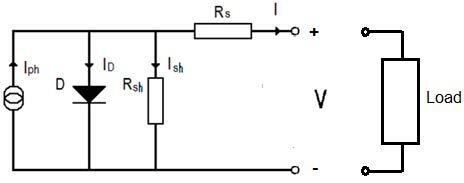
\includegraphics[width=0.7\textwidth]{figures/scheme.jpg}
		\caption[Scheme of solar cell]{Scheme of solar cell with current source, perfect diode, internal and load resistors.}
		\label{fig:scheme}
	\end{figure}

%On all scopes the x-axes is the time in seconds. The y-axes is declarated in each window.	

\section{Model Development}

	\subsection{Parameters}
	A .mat file has the advantage that it saves just variables. If you want to call variables in a .m file the whole skrip has to be calculated. This can be noticeable with many variables. See code in Listing \ref{code} Line 5-19.
	
	\newpage	
	\subsection{Interface}
	The irradiance can 't be influenced and is clearly an input.
	The solar cell delivers a power. A part of this power is losses in the cell itself. Depending on the irradiance [G] and the load, a different output voltage [V] and current [I] is established.
	Charging a battery requires a constant voltage [V]. Therefore, this is handled as an input and the current [I] as output.
	
		\begin{itemize}
			\item[$\Leftarrow$ [G]] Irradiance
			\item[$\Leftarrow$ [V]] Voltage
			\item[$\Rightarrow$ [I]] Current
		\end{itemize}
	

	%\newpage
	\subsection{Model Design}
	With the equations from Equation \ref{eq:1} - \ref{eq:4} was built a model of the system with subsystems.
	In Figure \ref{fig:overview} is an overview of the system. This topsystem represents Equation \ref{eq:1}. Each of the subsytems symbolizes one of the  Equations \ref{eq:2} - \ref{eq:4}. Details of the subsystems are visible in Figure \ref{fig:i_ph} - \ref{fig:i_d}.

		\begin{figure}[H]
			\centering
			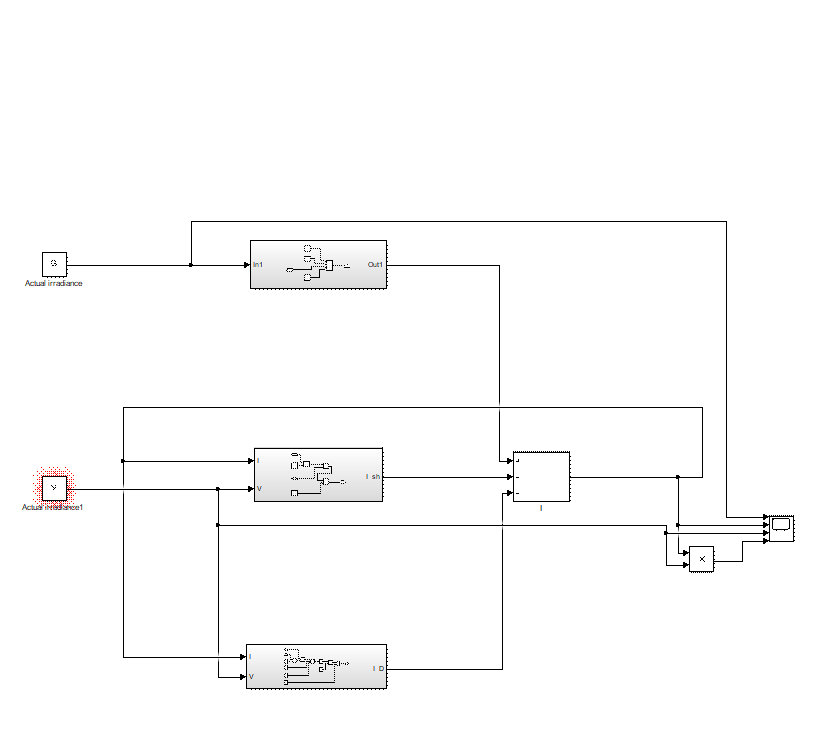
\includegraphics[width=0.7\textwidth]{figures/overview.png}
			\caption{Mathematical overview scheme based on the Equations \ref{eq:1} - \ref{eq:4}}
			\label{fig:overview}
		\end{figure}
	
		\begin{figure}[H]
			\centering
			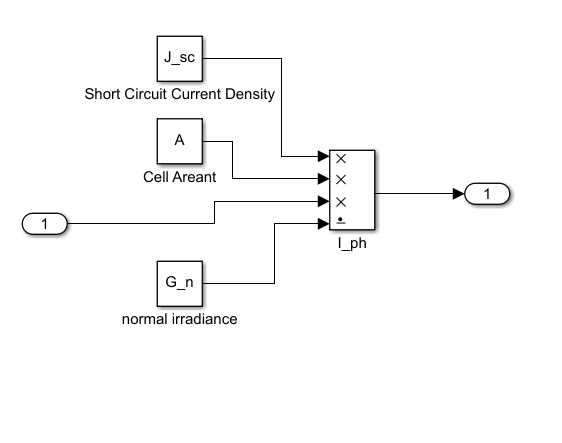
\includegraphics[width=0.7\textwidth]{figures/i_ph.png}
			\caption[The total current of the irradiance without losses.]{The total current of the irradiance without losses. The top block on Figure \ref{fig:overview}.}
			\label{fig:i_ph}
		\end{figure}
	
		\begin{figure}[H]
			\centering
			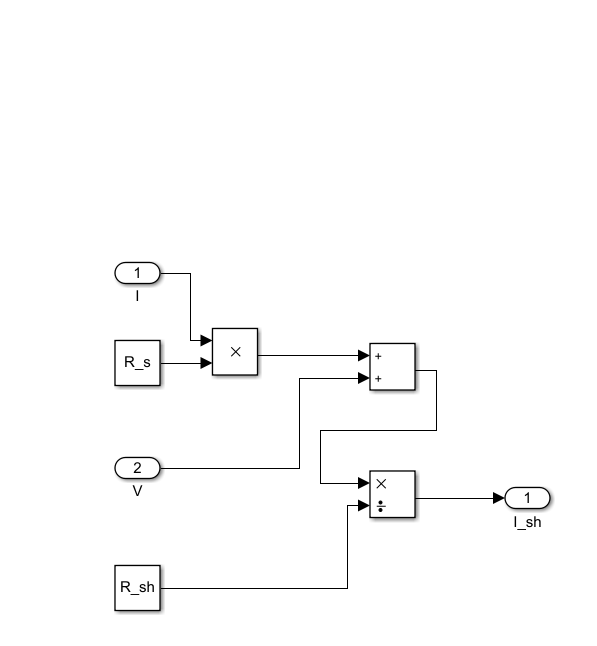
\includegraphics[width=0.7\textwidth]{figures/i_sh.png}
			\caption[Loss current from the internal resistance.]{Loss current from the internal resistance. The block in the middle on Figure \ref{fig:overview}.}
			\label{fig:i_sh}
		\end{figure}
	
		\begin{figure}[H]
			\centering
			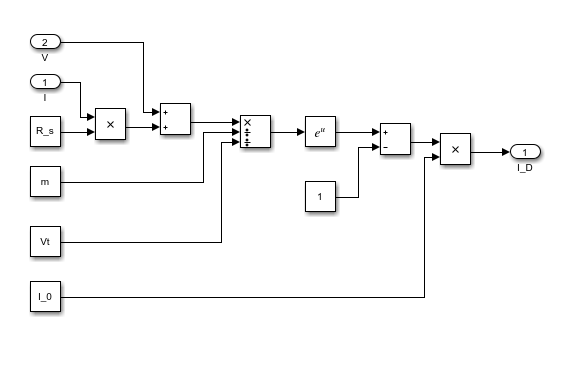
\includegraphics[width=0.7\textwidth]{figures/i_d.png}
			\caption[Loss current of the diode.]{Loss current of the diode. The bottom block on Figure \ref{fig:overview}}
			\label{fig:i_d}
		\end{figure}
	
	\subsection{Simulation}
	There where no warnings. Everything is fine.

\newpage
\section{Model Testing}
For the following simulations the irradiance was fixed at $1000^W/_{m^2}$.
On all scopes the x-axes is the time in seconds. The y-axes are declarated in each window.

\newpage
	
	\subsection{Short Circuit}
	In the event of a short circuit, the output voltage is set to 0V. In Figure \ref{fig:shortc} are the graphes with the values visible.
	The total power is increased over the resistances $R_s$ and $R_{sh}$. The current is visible on Figure \ref{fig:shortc} and is approximately 4.35A. A higher irradiance delievers a higher short circuit current. More about the influence of irradiance in Section \ref{sec:irra}.
	
		\begin{figure}[H]
			\centering
			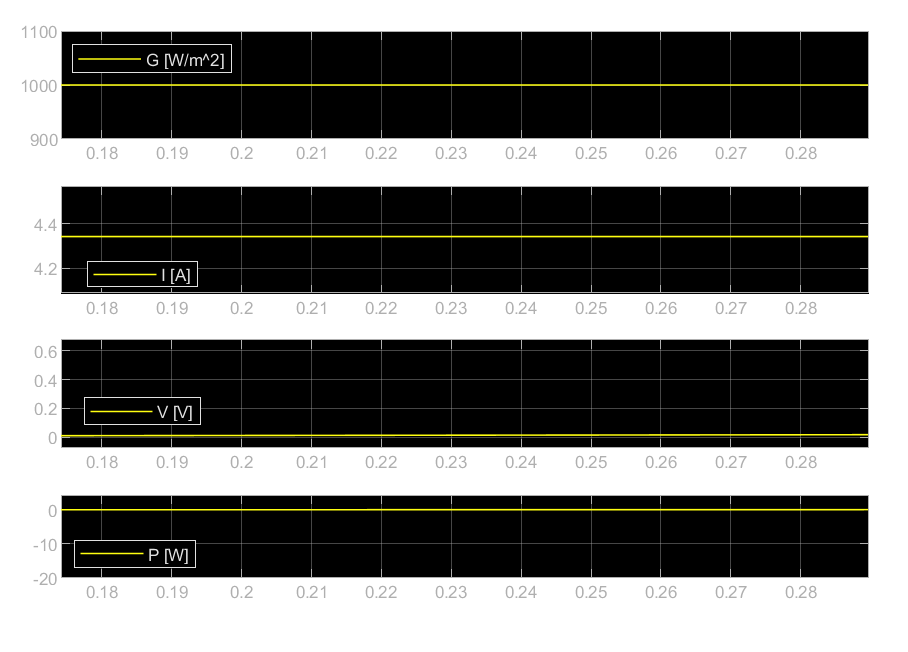
\includegraphics[width=0.7\textwidth]{figures/shortcircuit.eps}
			\caption[The scope arround the point of a short circuit with irradiance  of $1000^W/_{m^2}$.]{The scope arround the point of a short circuit with irradiance  of $1000^W/_{m^2}$. On all scopes the x-axes is the time in seconds. The y-axes is declarated in each window.}
			\label{fig:shortc}
		\end{figure}
	
	\subsection{Open Circuit}
	When no load is connected, the whole power is increased over $R_{sh}$. The current I is 0A. The values can be read in Figure \ref{fig:openc} at the place where the current crosses the 0A line. The voltage at this point is about 0.455V.
		
		\begin{figure}[H]
			\centering
			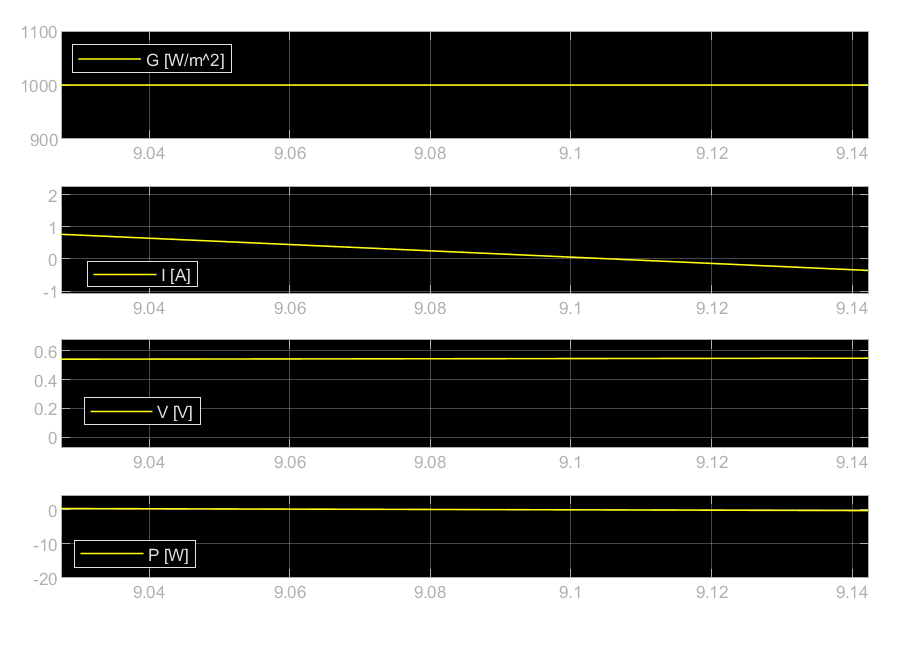
\includegraphics[width=0.7\textwidth]{figures/opencircuit.eps}
			\caption{The scpoe arraound the point of an open circuit with irradiance  of $1000^W/_{m^2}$.}
			\label{fig:openc}
		\end{figure}
	
	\subsection{Open Circuit with a higher Voltage}
	If the voltage raises further  the current get negative and the power too. That means the solar cell can 't deliver more then this approximately 0.455V by an irradiance of 1000$^W/_{m^2}$. This is visible in Figure \ref{fig:allg}.
	
	\subsection{Open Circuit with a higher Irradiance}
	If the irradiance is increased to 1500$^W/_{m^2}$, a higher output voltage will occur. This is visible on Figure \ref{fig:openc1500} where the voltage is about 0.55V. More about this topis in Section \ref{sec:irra}.
	
		
		\begin{figure}[H]
			\centering
			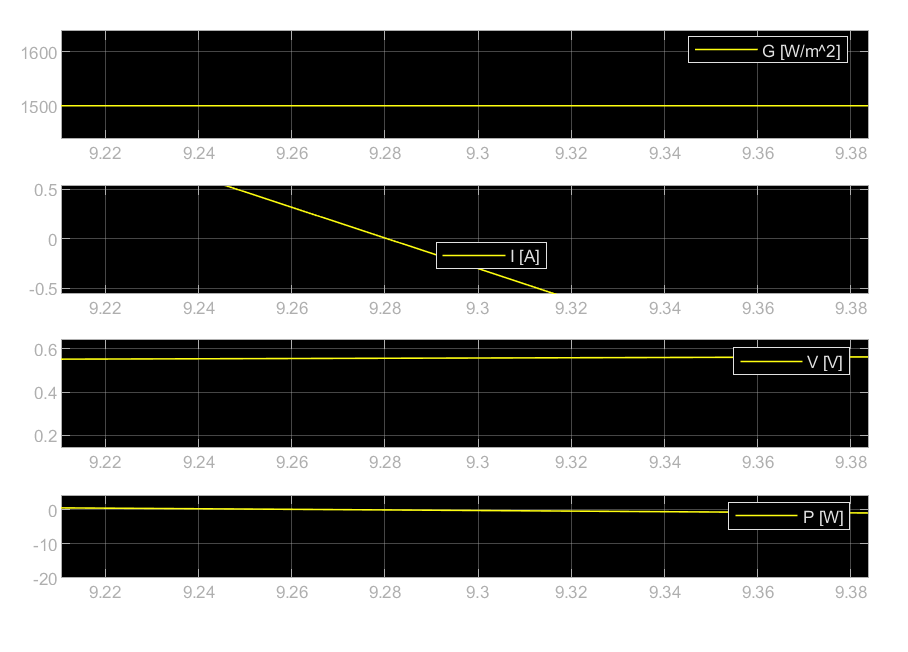
\includegraphics[width=0.7\textwidth]{figures/openc1500.eps}
			\caption{The scpoe arraound the point of an open circuit with irradiance  of $1500^W/_{m^2}$.}
			\label{fig:openc1500}
		\end{figure}
	
	\subsection{Storing of simulation results}
	The loged datas will be stored in a Struct. Each port has the properties:
		\begin{itemize}
			\item PortType
			\item PortIndex
			\item PropagatedName
			\item Blockpath
			\item Values
			\item Name
		\end{itemize}
	
	Each value is logged every 0.2 seconds. The Figure \ref{fig:plot} is made with the loged datas after the resistance ramp was removed. The resistance and the power graphs are calculated with voltage and current. See Listing \ref{code} Line 25-56.
	
		\begin{figure}[H]
			\centering
			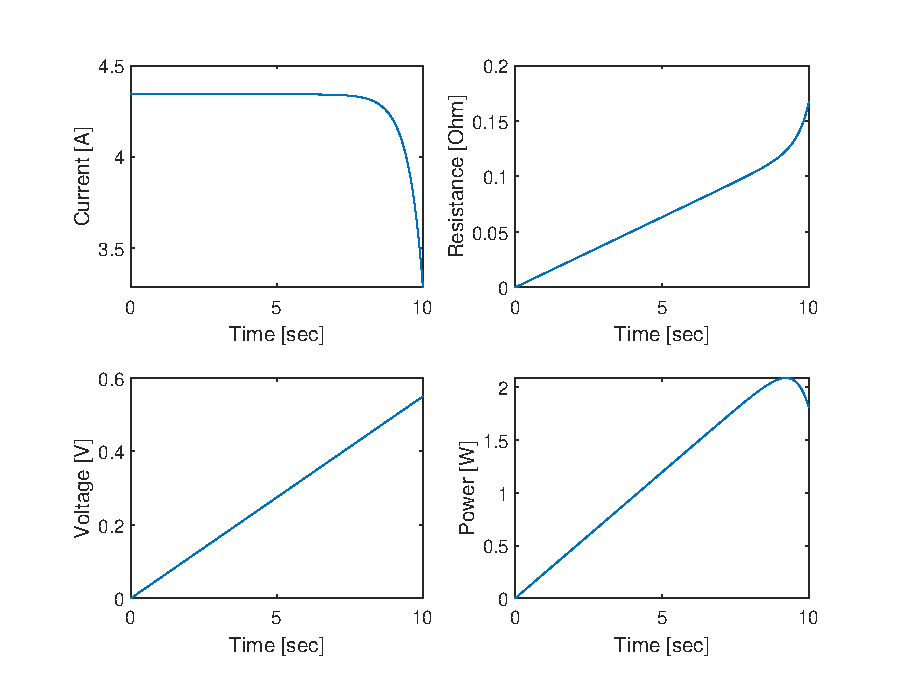
\includegraphics[width=0.7\textwidth]{figures/logplot.eps}
			\caption{The ploted graph is made with the loged datas.}
			\label{fig:plot}
		\end{figure}
	
	
	
	\subsection{Characteristic curves of the solar cell}
	The simulink model (Figure \ref{fig:over2}) was extended with a variable $R_{Load}$ as a ramp with a slope of 0.1$^{\Omega}/_{s}$. The voltage V was defined as product of $R_{Load}$ and I. The $R_{Load} $was added to the scoap in Figure \ref{fig:var_r}.\\
	It is clear visible that the current becomes smaller after about one second with greater resistance and the voltage first rises quickly and goes to saturation at about 5.5V from about 1.25 seconds.
	The power has its peak of almost 2W at about 1.25 seconds.
		
		\begin{figure}[H]
			\centering
			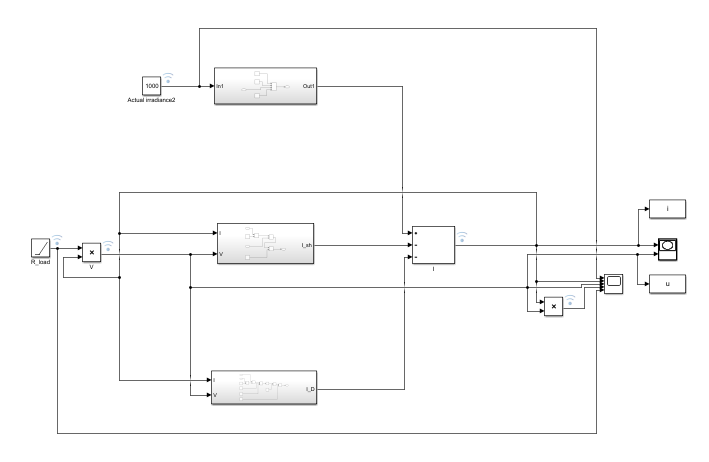
\includegraphics[width=0.7\textwidth]{figures/over2.png}
			\caption[The voltage defined as product of I and $R_{Load}$.]{The voltage defined as product of I and $R_{Load}$. The variables V and I where recorded as array in Matlab. Visible on the right side of the figure, next to an XY-Scope.}
			\label{fig:over2}
		\end{figure}	
		
		\begin{figure}[H]
			\centering
			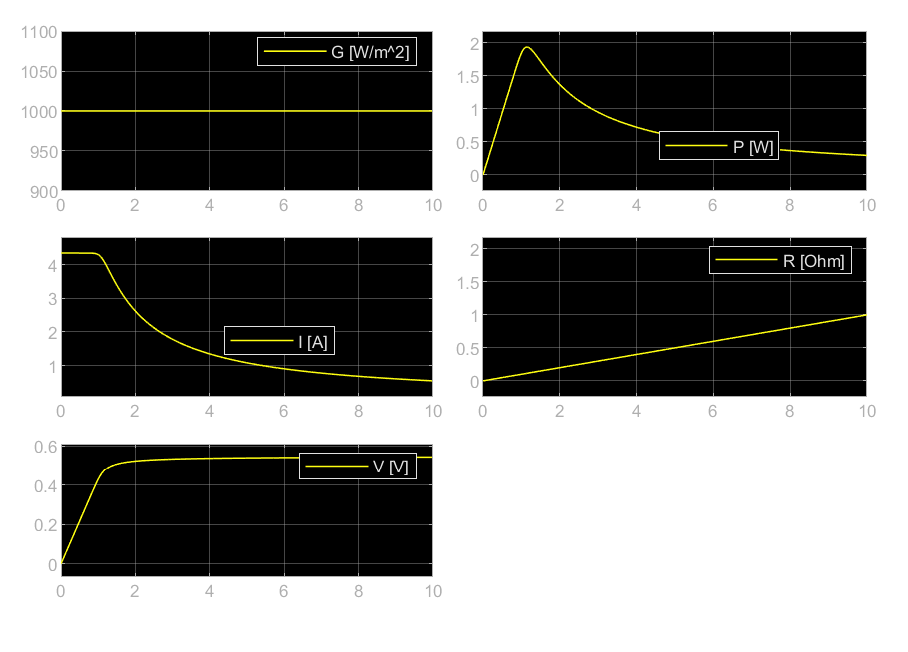
\includegraphics[width=0.7\textwidth]{figures/var_r.eps}
			\caption{The extended scope with $R_{Load}$.}
			\label{fig:var_r}
		\end{figure}
	In Figure \ref{fig:xy} is the dependence between current and voltage. 
	The goal is to find the point with the largest area with the product of voltage and current.
	This can be seen more easily in Figure \ref{fig:var_r} as peak of the power in the graph top right.
	
		\begin{figure}[H]
			\centering
			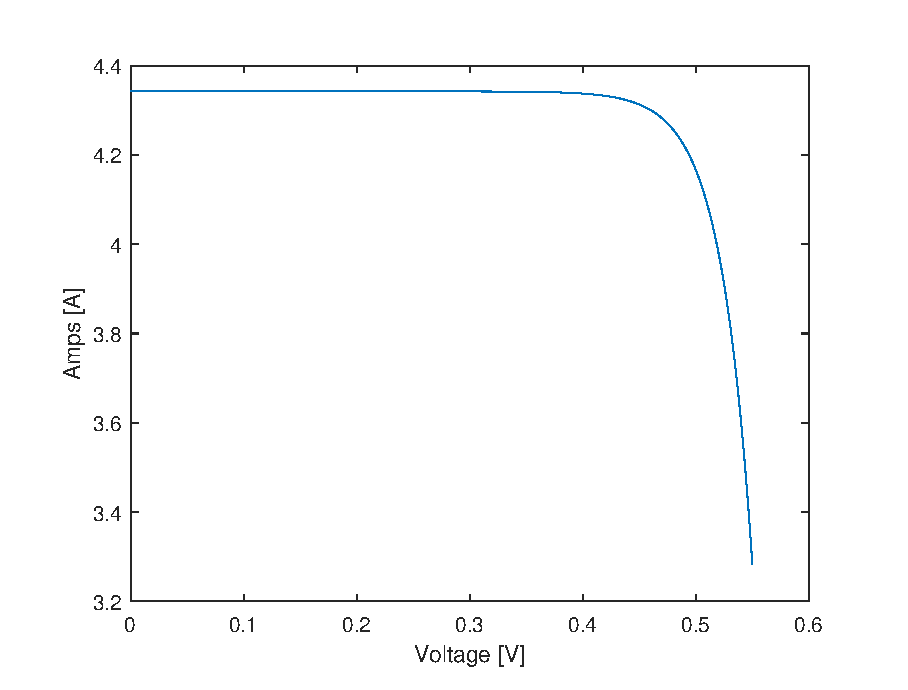
\includegraphics[width=0.7\textwidth]{figures/xy.eps}
			\caption{XY-Plot with voltage and current. The product of current and voltage from each point on the line is the resulting power in watt.}
			\label{fig:xy}
		\end{figure}
	

%	U Bereich, U für Max P...
%	\begin{figure}[H]
%		\centering
%		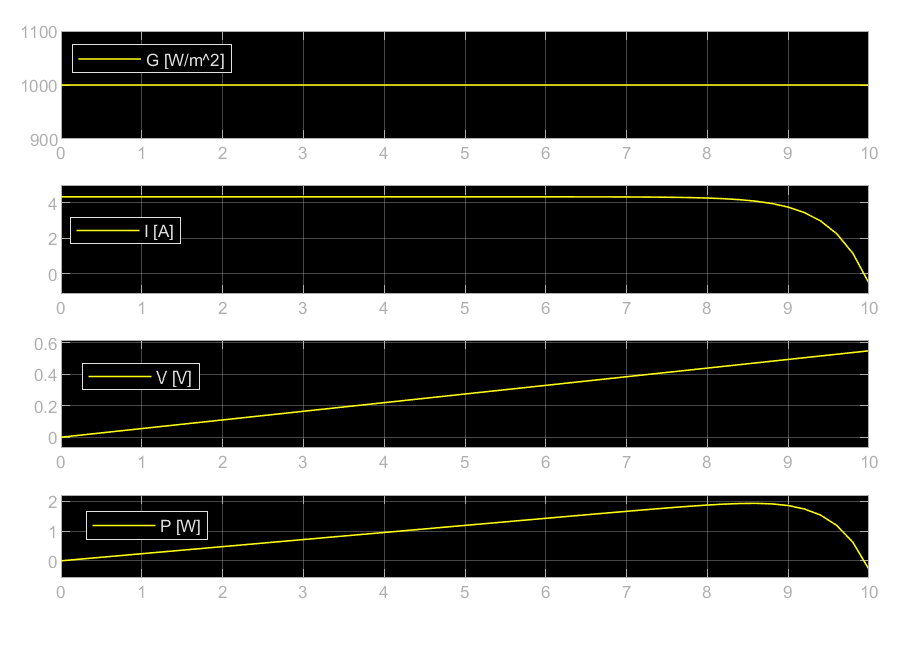
\includegraphics[width=0.7\textwidth]{figures/ramp_v.eps}
%		\caption{...}
%		\label{fig:ramp_v}
%	\end{figure}
%
%	\begin{figure}[H]
%		\centering
%		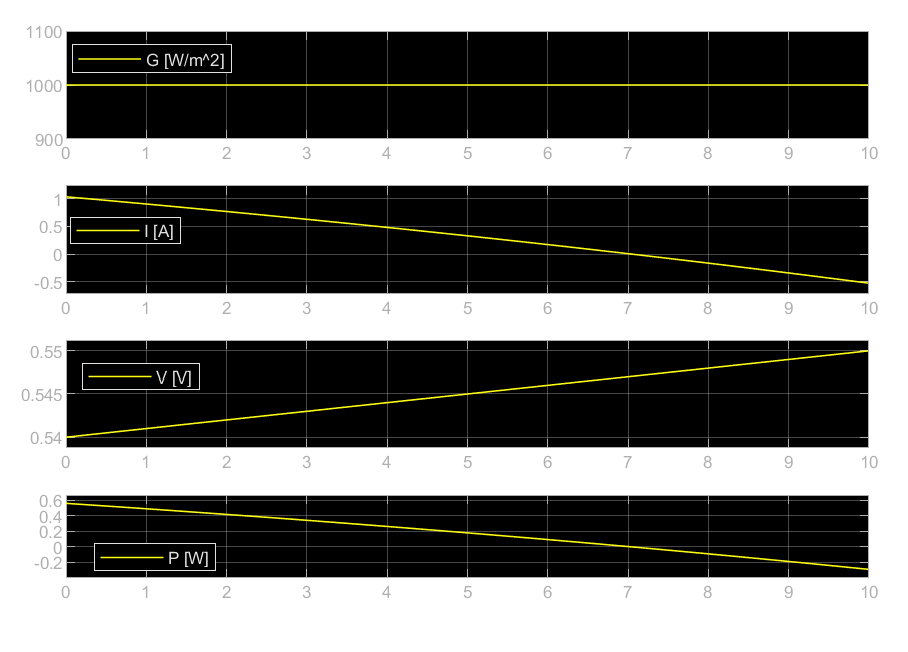
\includegraphics[width=0.7\textwidth]{figures/ramp_v_zoom.eps}
%		\caption{...}
%		\label{fig:ramp_vzoom}
%	\end{figure}

	

\newpage
\section{Irradiance effect on solar cell performance} \label{sec:irra}

	\subsection{Temperature}
	The thermal voltage was already set at the start of the laboratory unit to 25.85V at 300K. The difference of a $\Delta$T of 1.85K is unknown. More on this topic in Section \ref{sec:temp}.
	
	\subsection{Variable Irradiance}
	On the following Figures \ref{fig:g400} - \ref{fig:g1200} the irradiance was varied. All other settings have been retained. The scaling of the plots is also the same in all figures.
	On Figure \ref{fig:allg} is an current voltage plot overview with all irradiances. On Figure \ref{fig:xy_vp} is an overview with power and voltage with different irradiances. The Matlab code for Figure \ref{fig:allg} and Figure \ref{fig:xy_vp} is in Listing \ref{code} Line 66 - 126.
		
		\begin{figure}[H]
			\centering
			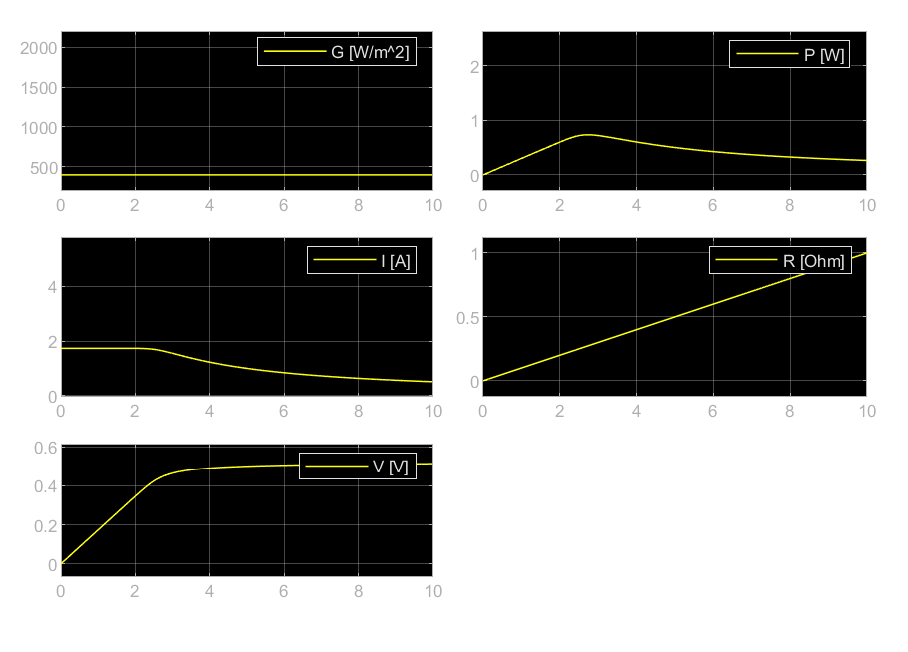
\includegraphics[width=0.7\textwidth]{figures/g400.eps}
			\caption{Fixed irradiance at 400 $^W/_{m^2}$ with a variable resistance as ramp from 0-1$\Omega$}
			\label{fig:g400}
		\end{figure}
		\begin{figure}[H]
			\centering
			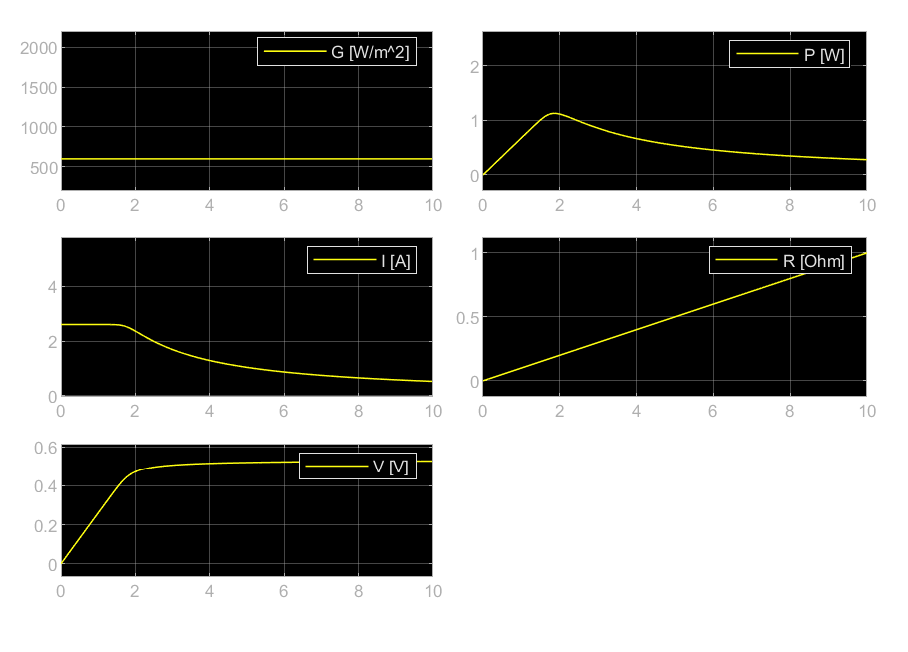
\includegraphics[width=0.7\textwidth]{figures/g600.eps}
			\caption{Fixed irradiance at 600 $^W/_{m^2}$ with a variable resistance as ramp from 0-1$\Omega$}
			\label{fig:g600}
		\end{figure}	
		\begin{figure}[H]
			\centering
			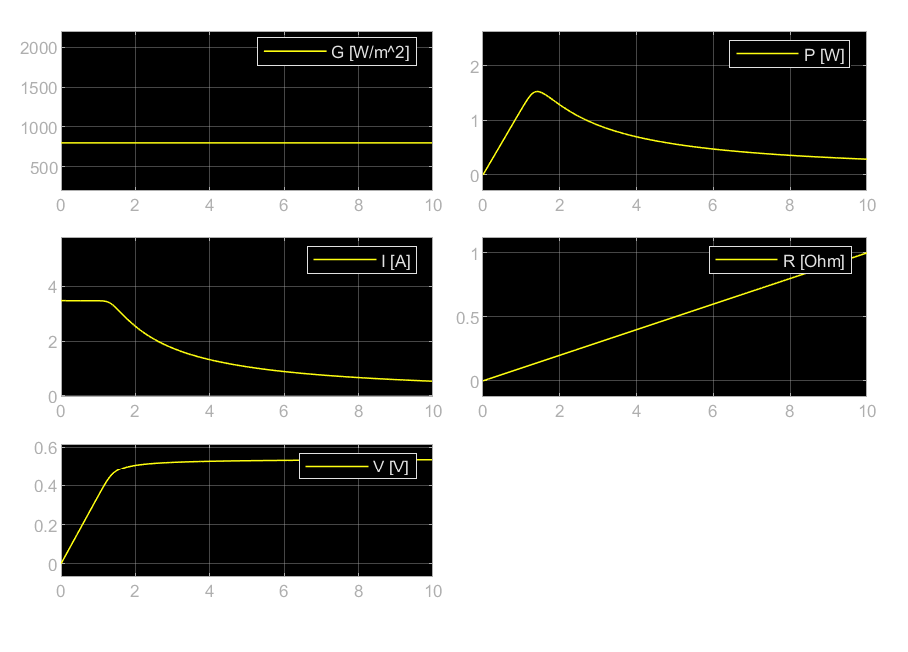
\includegraphics[width=0.7\textwidth]{figures/g800.eps}
			\caption{Fixed irradiance at 800 $^W/_{m^2}$ with a variable resistance as ramp from 0-1$\Omega$}
			\label{fig:g800}
		\end{figure}	
		\begin{figure}[H]
			\centering
			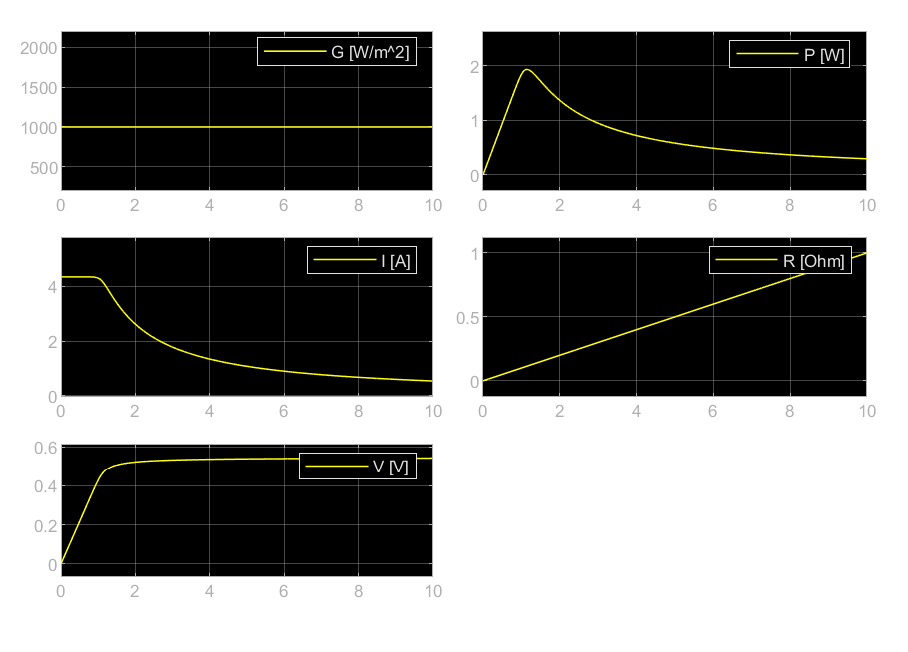
\includegraphics[width=0.7\textwidth]{figures/g1000.eps}
			\caption{Fixed irradiance at 1000 $^W/_{m^2}$ with a variable resistance as ramp from 0-1$\Omega$}
			\label{fig:g1000}
		\end{figure}	
		\begin{figure}[H]
			\centering
			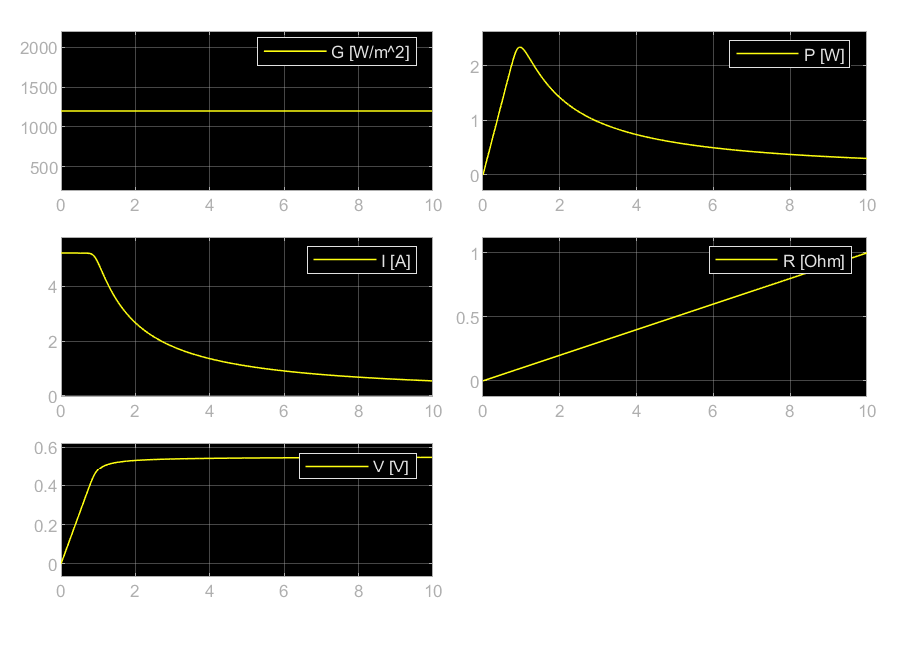
\includegraphics[width=0.7\textwidth]{figures/g1200.eps}
			\caption{Fixed irradiance at 1200 $^W/_{m^2}$ with a variable resistance as ramp from 0-1$\Omega$}
			\label{fig:g1200}
		\end{figure}	
		\begin{figure}[H]
			\centering
			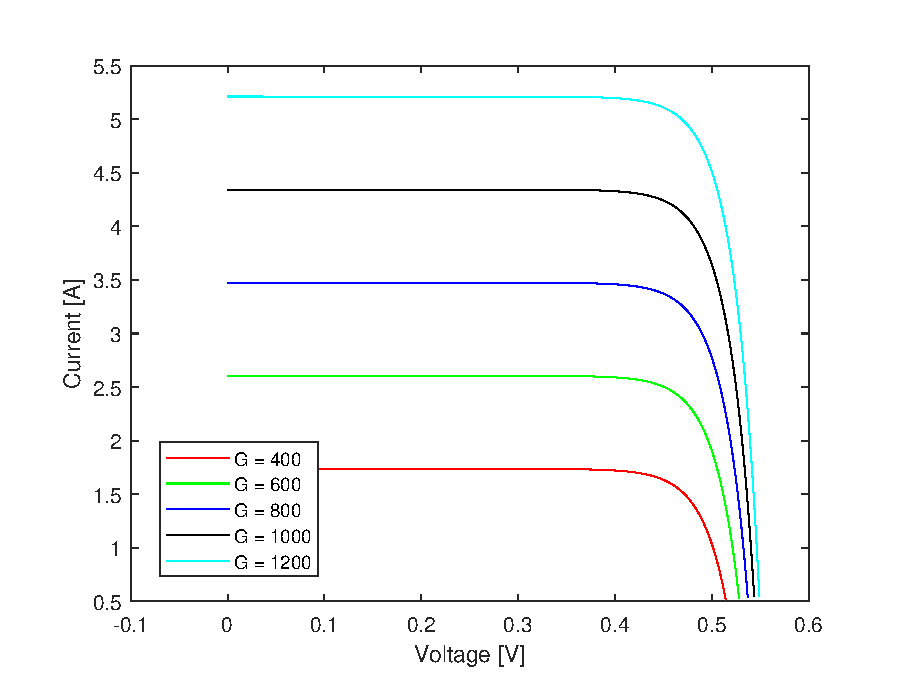
\includegraphics[width=0.7\textwidth]{figures/g_in_one.eps}
			\caption[Current dipence on voltage.]{Current dipence on voltage. The different lines symbolizes different irradiances G.}
			\label{fig:allg}
		\end{figure}
	
	\subsection{Maximum Power Point}
	On the following Figures \ref{fig:max1} and \ref{fig:max2} are an XY-plot of current and voltage next to a XY-plot of voltage and power. The scale is different on each plot to make the Maximum Power Point better visible. On the last Figure \ref{fig:xy_vp} is an overview of all Maximum Power Points from the different irradiances. The Matlab code is in Listing \ref{code} Line131 - 145.
	

	
		\begin{figure}[H]
		\begin{center}
			\begin{subfigure}{0.4\textwidth}
			\begin{center}
				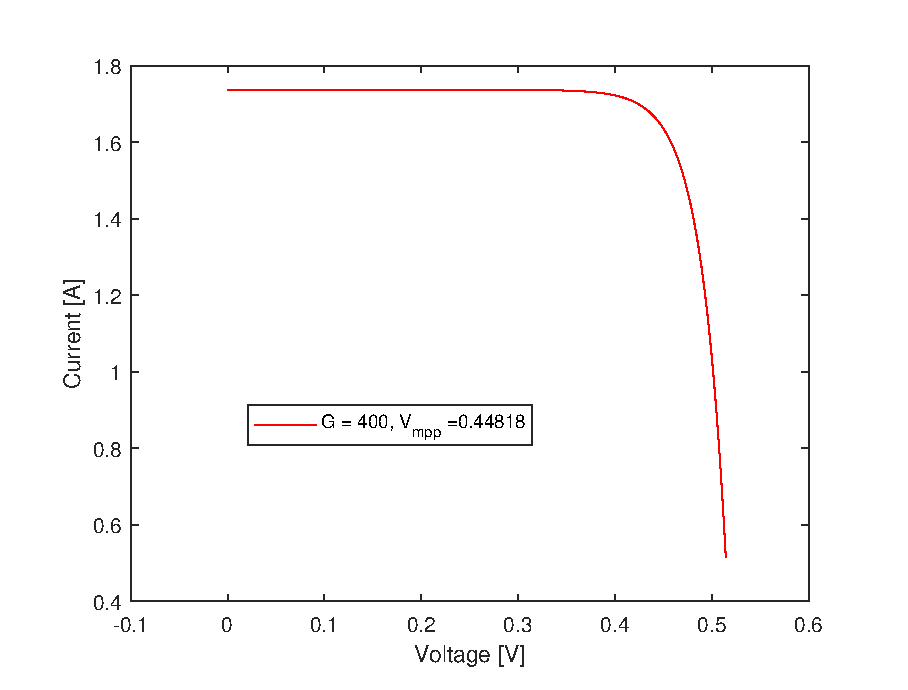
\includegraphics[width=1\textwidth]{figures/vg400.eps}
			\end{center}	
			\end{subfigure}
			\begin{subfigure}{0.4\textwidth}
				\begin{center}
					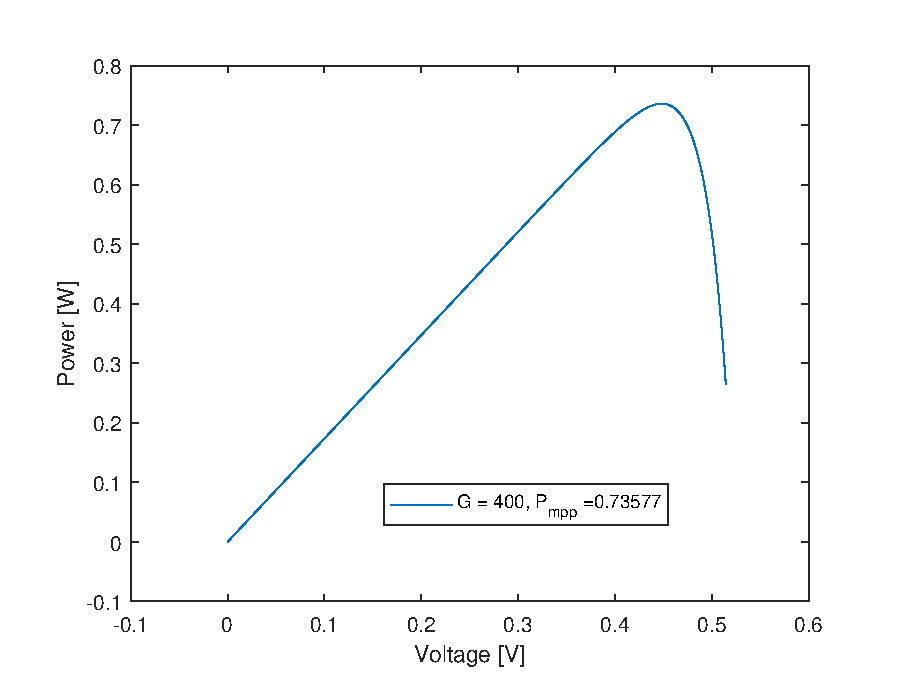
\includegraphics[width=1\textwidth]{figures/pg400.eps}
				\end{center}	
			\end{subfigure}
			\begin{subfigure}{0.4\textwidth}
				\begin{center}
					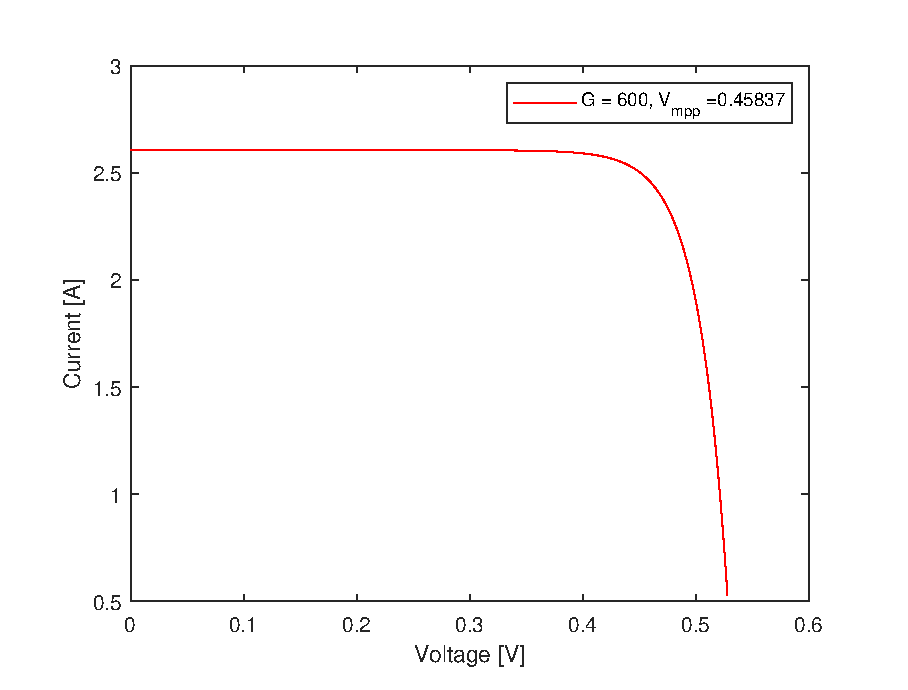
\includegraphics[width=1\textwidth]{figures/vg600.eps}
				\end{center}	
			\end{subfigure}
			\begin{subfigure}{0.4\textwidth}
				\begin{center}
					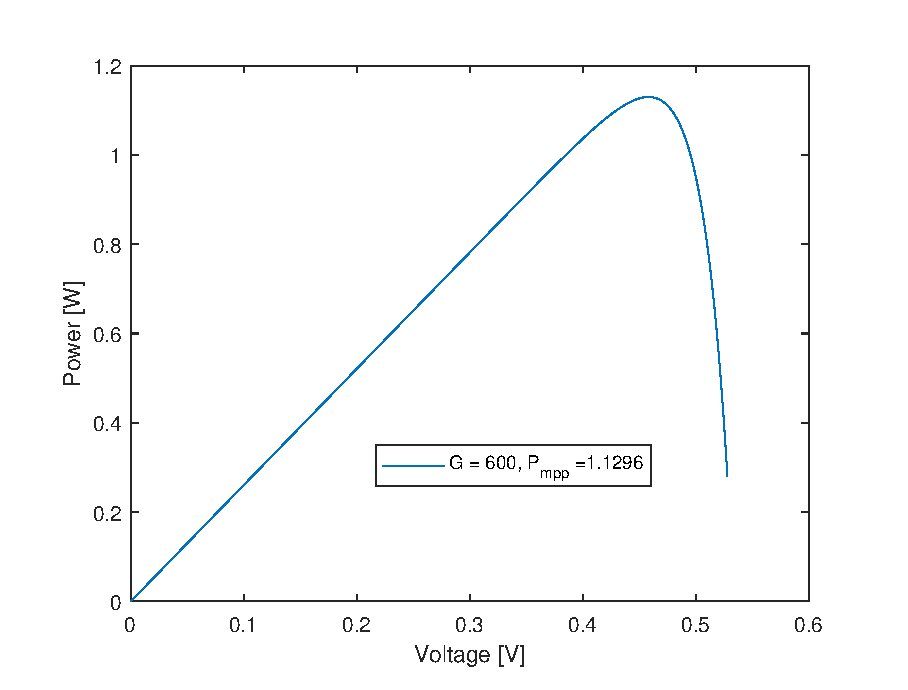
\includegraphics[width=1\textwidth]{figures/pg600.eps}
				\end{center}	
			\end{subfigure}
			\begin{subfigure}{0.4\textwidth}
				\begin{center}
					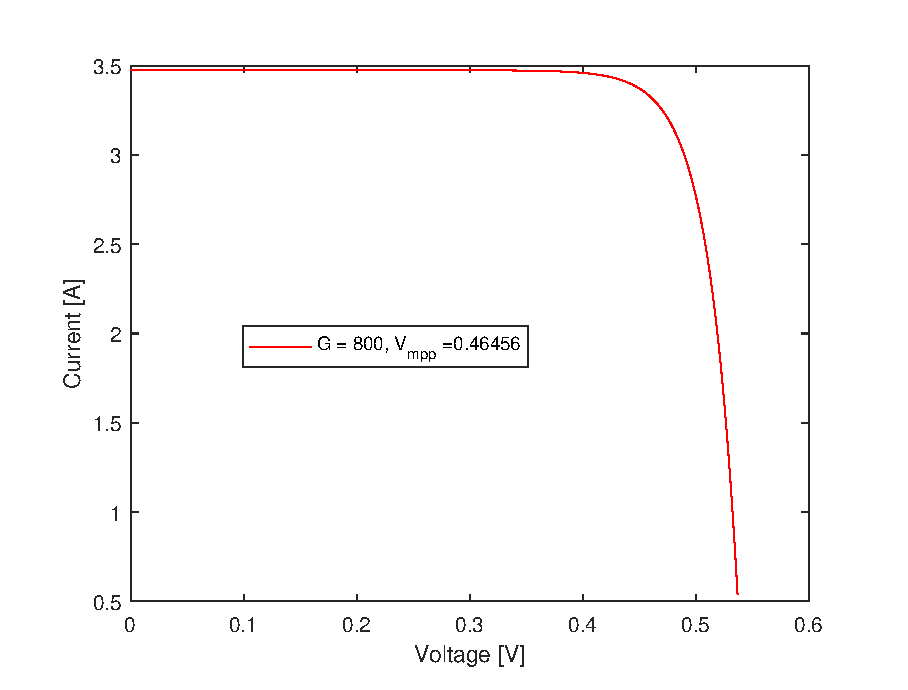
\includegraphics[width=1\textwidth]{figures/vg800.eps}
				\end{center}	
			\end{subfigure}
			\begin{subfigure}{0.4\textwidth}
				\begin{center}
					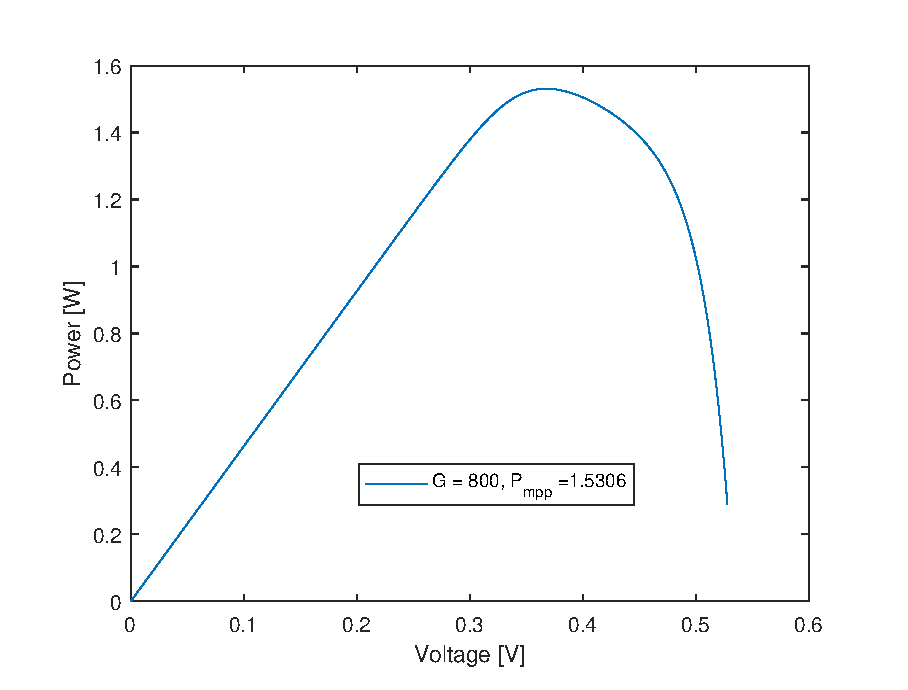
\includegraphics[width=1\textwidth]{figures/pg800.eps}
				\end{center}	
			\end{subfigure}
			\caption{Maximum Power Point, G = 400, 600, 800\\ 1 of 2}
			\label{fig:max1}
		\end{center}
		\end{figure}
	
		\begin{figure}[H]		
		\begin{center}
			\begin{subfigure}{0.4\textwidth}
				\begin{center}
					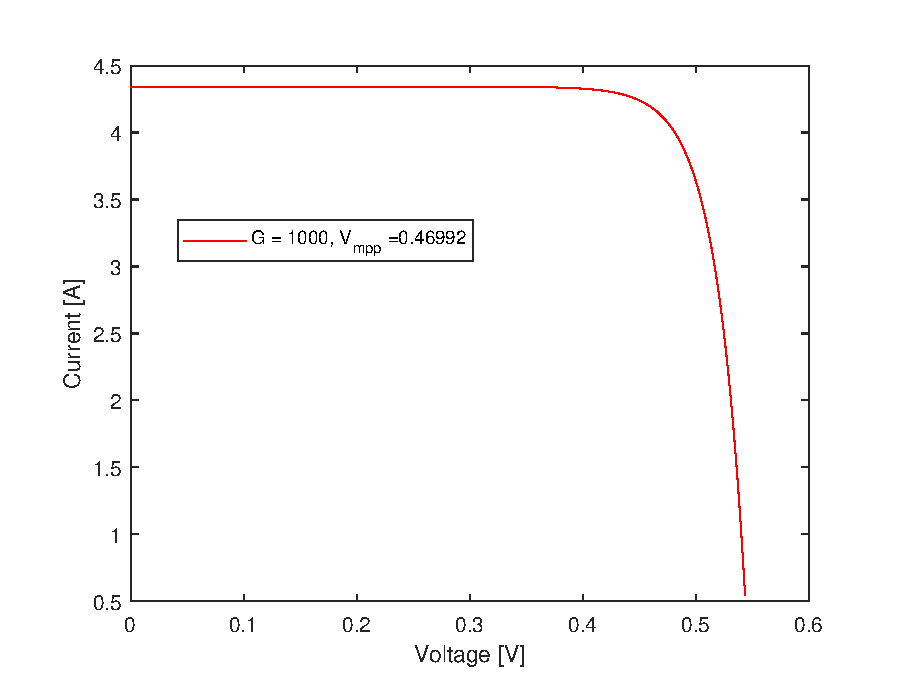
\includegraphics[width=1\textwidth]{figures/vg1000.eps}
				\end{center}	
			\end{subfigure}
			\begin{subfigure}{0.4\textwidth}
				\begin{center}
					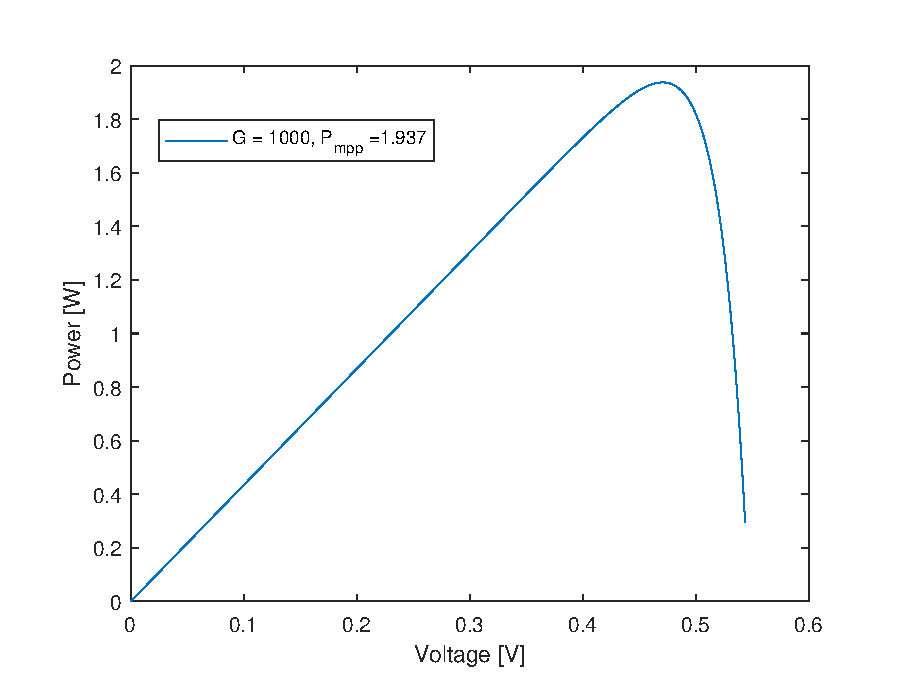
\includegraphics[width=1\textwidth]{figures/pg1000.eps}
				\end{center}	
			\end{subfigure}
			\begin{subfigure}{0.4\textwidth}
				\begin{center}
					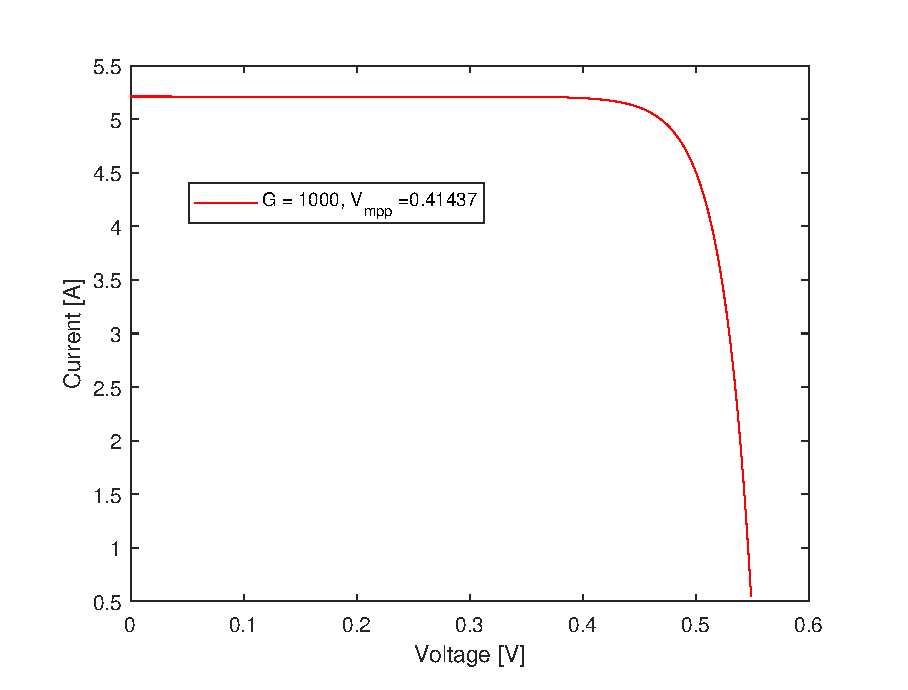
\includegraphics[width=1\textwidth]{figures/vg1200.eps}
				\end{center}	
			\end{subfigure}
			\begin{subfigure}{0.4\textwidth}
				\begin{center}
					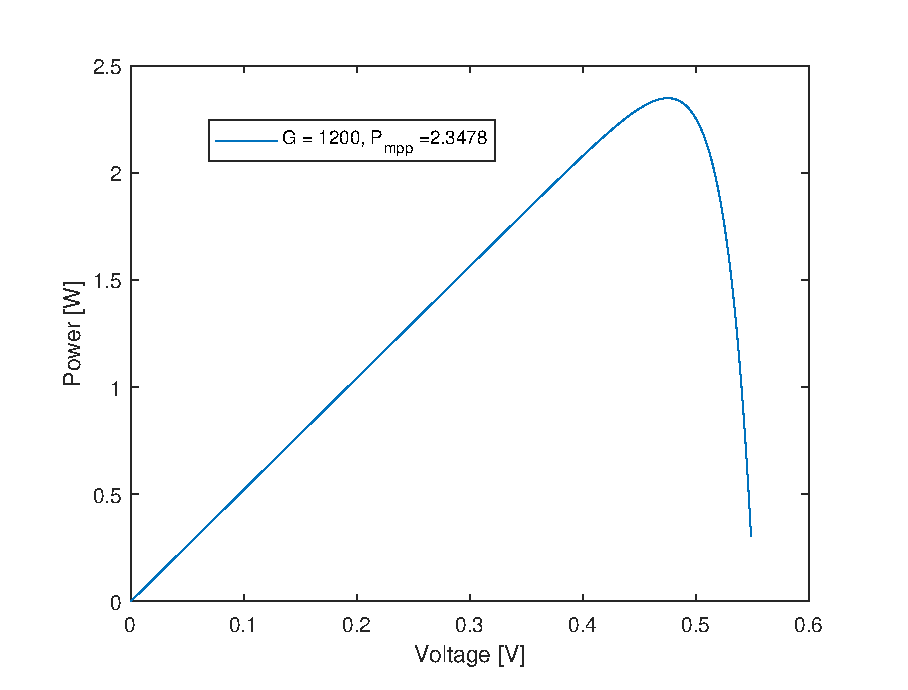
\includegraphics[width=1\textwidth]{figures/pg1200.eps}
				\end{center}	
			\end{subfigure}
			\caption{Maximum Power Point, G = 1000, 1200\\ 2 of 2}
			\label{fig:max2}
		\end{center}
		\end{figure}
	
		\begin{figure}[H]
			\centering
			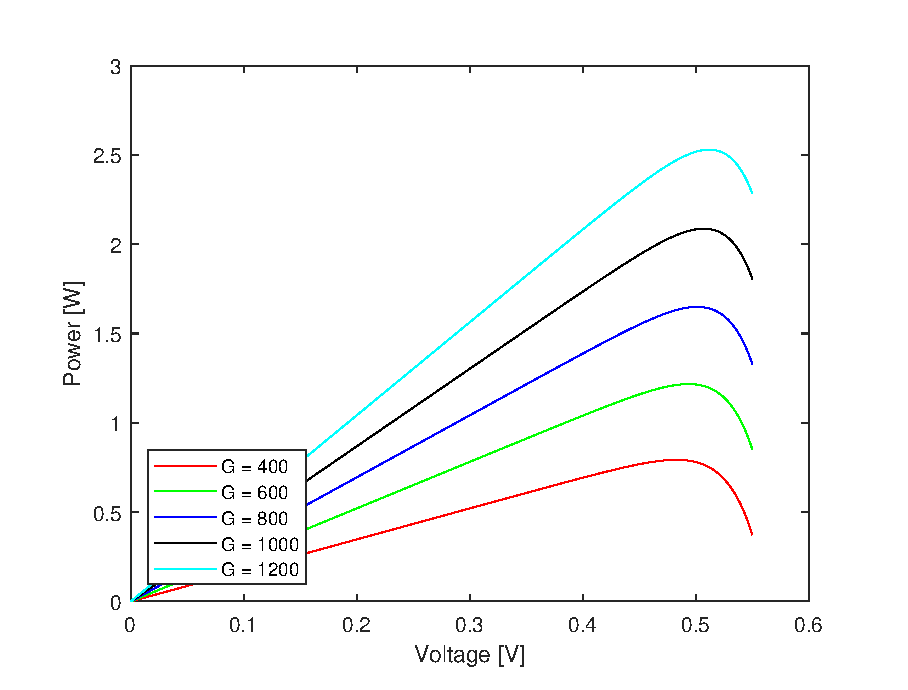
\includegraphics[width=0.7\textwidth]{figures/xy_vp.eps}
			\caption{Power depence on voltage. The different lines symbolizes different irradiances G.}
			\label{fig:xy_vp}
		\end{figure}

\newpage
\section{Lookup table creation}
In the Tables \ref{tb:arr1} and \ref{tb:arr2} are two examples of lookup tables. Table \ref{tb:arr1} is two dimensional with two inputs. 
Table \ref{tb:arr2} is like in the task with voltage as input and current as output. This lookup tables are just for visualisation. So there are less values in it. The code to built these two  Arrays is in Listing \ref{code} Line 148 - 180.\\
With the commad tic and toc would be stoped the simulation time from the code in Listing \ref{code} Line 64 - 97. The stoped time was 6.9 seconds. The model was simulated five times with different irradiances. The averrage for each simulation is so $\frac{6.9s}{5} = 1.4s$. \\
The next step was to comment out the saves to the arrays and measure the time again. This total time was 6.6s. Thats 1.3s per simulation. Not a big difference to the preview time.\\
Finally, the time was measured to read the array. The result was 0.03s and much smaller then one simulation run. The measurements are not very meaningful and are difficult to reproduce. \\
The advantage is that if the data is often needed, the simulation does not always have to be restarted. Thats saves time and energy. This is helpful in simulations which often have to be repeated.


	\begin{center}
	$\begin{array}{c|cccccccc}
		 & 0\Omega & 40m\Omega & 80m\Omega & 120m\Omega & 160m\Omega & 200m\Omega & 240m\Omega & 280m\Omega \\ \hline \rowcolor{lgray}
		 400^W/_{m^2} & 0 & 0.1207 & 0.2413 & 0.3619 & 0.4825 & 0.6018 & 0.7049 & 0.7347\\
		 600^W/_{m^2} & 0 & 0.2715 & 0.543 & 0.8141 & 1.0657 & 1.1161 & 1.015 & 0.9055\\ \rowcolor{lgray}
		 800^W/_{m^2} & 0 & 0.4827 & 0.9652 & 1.427 & 1.4834 & 1.2872 & 1.1107 & 0.971\\	 
		 1000^W/_{m^2} & 0 & 0.7542 & 1.5069 & 1.9265 & 1.6412 & 1.3686 & 1.1648 & 1.0114\\ \rowcolor{lgray}
		 1200^W/_{m^2} & 0 & 1.086 & 2.1503 & 2.1538 & 1.7291 & 1.4216 & 1.2026 & 1.0407 
	\end{array}$
	\captionof{table}{Lookup Table with G and $R_{Load}$ as input and P as output}
	\label{tb:arr1}
	\end{center}

	\begin{center}
		$\begin{array}{c|cccccccc} 
			Voltage \left[ V\right] & 0 & 0.022 & 0.044 & 0.066 & 0.088 & 0.11 & 0.132 & 0.154 	\\ \hline \rowcolor{lgray}
			Current \left[ A\right] & 4.3424 & 4.3424 & 4.3423 & 4.3423 & 4.3423 & 4.3423 & 4.3422 & 4.3422		
		\end{array}$
		\captionof{table}{Lookup Table with G and $R_{Load}$ as input and P as output}
		\label{tb:arr2}
	\end{center}




\newpage
\section{Temperature Effect on PV Performance}\label{sec:temp}
In this section, the influence of temperature was included. For this purpose, the simulink model was adjusted as shown in Figure \ref{fig:i_d2}.
The model was simulated with the temperatures 15°C, 20°C, 30°C, 40°C and 50°C. The values were converted from Celsius to Kelvin for the Input. The code is in Listing \ref{code} Line 186 - 241.


	\begin{figure}[H]
		\centering
		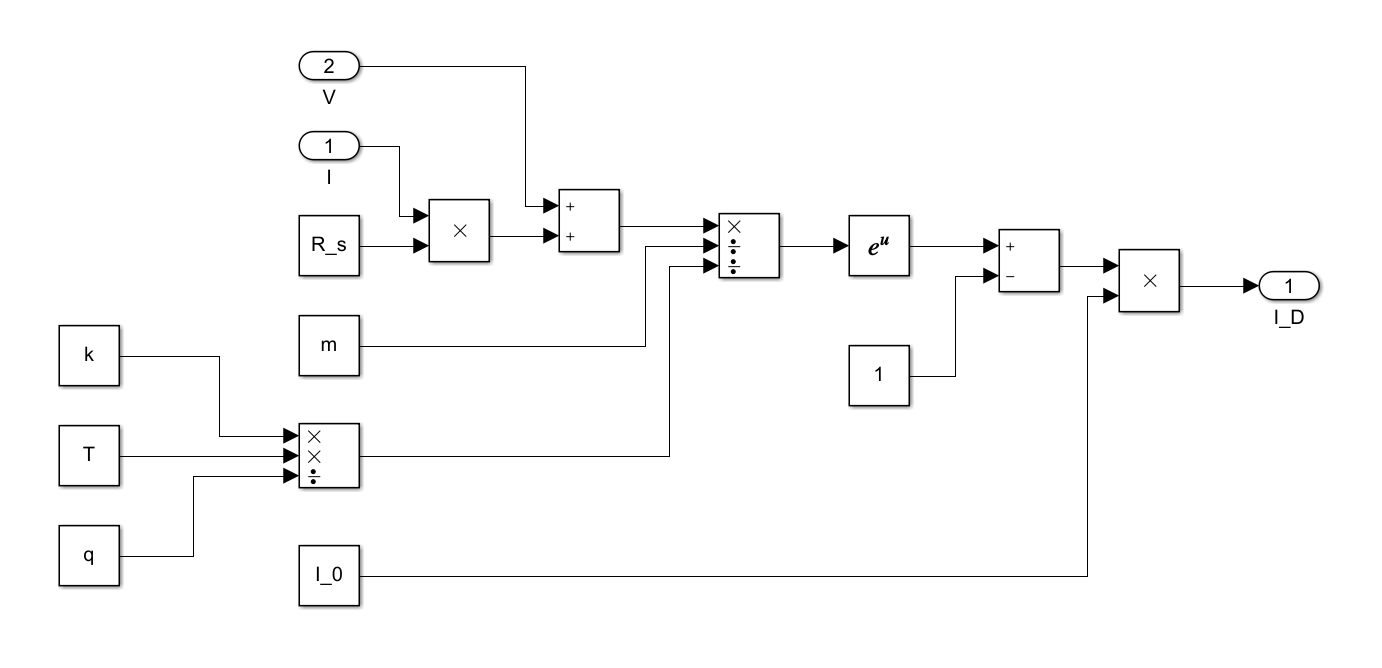
\includegraphics[width=0.7\textwidth]{figures/i_ph_2.png}
		\caption{Update of the Figure \ref{fig:i_d}. Now with the influence of temperature.}
		\label{fig:i_d2}
	\end{figure}
In Figure \ref{fig:xy_vc_t} and \ref{fig:xy_vp_t} are the plots with current and power depending on the voltage at different temperatures.
Mathematically, it is true that the output power increases with higher temperature. Because $V_t$ gets bigger with increasing temperature T.
	\begin{equation}
		T_t = \frac{k * T}{q}
	\end{equation}
The larger $V_t$ effects that the loss current become smaller. This can be seen in Equation \ref{eq:id}. The plots prove this calculation, seen in Figure \ref{fig:xy_vc_t} and \ref{fig:xy_vp_t}. On this  figures is also visible that that the influence is only visible with a large $R_{load}$.
However, this is not what can be expected physicaly. Solar cells produces more energy by lower temperatures \cite{tiez} \cite{pv}.

	\begin{figure}[H]
		\centering
		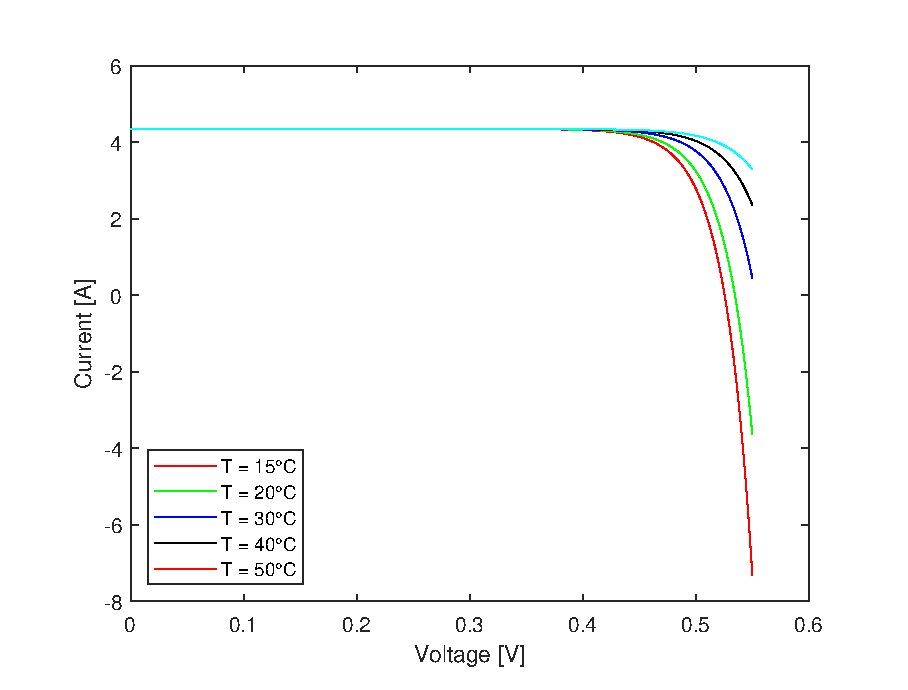
\includegraphics[width=0.7\textwidth]{figures/xy_vc_t.eps}
		\caption[Current dipence on Voltage with a constant irradiance and different temperatures]{Current dipence on Voltage with a constant irradiance. The different lines are the different temperatures 15°C, 20°C, 30°C, 40°C and 50°C.}
		\label{fig:xy_vc_t}
	\end{figure}

	\begin{figure}[H]
		\centering
		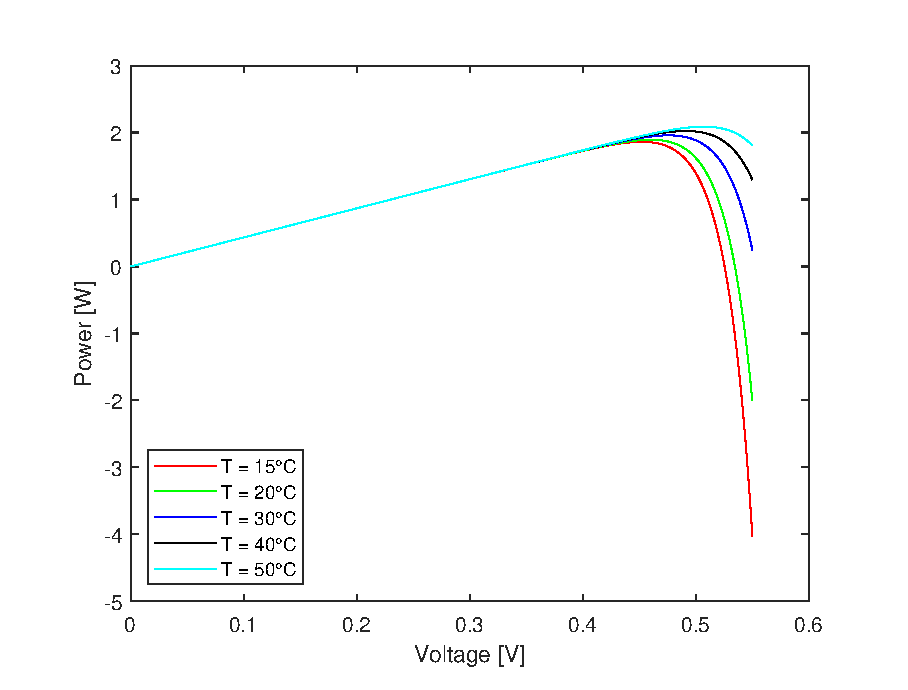
\includegraphics[width=0.7\textwidth]{figures/xy_vp_t.eps}
		\caption[Power dipence on Voltage with a constant irradiance.]{Power dipence on Voltage with a constant irradiance. The different lines are the different temperatures 15°C, 20°C, 30°C, 40°C and 50°C.}
		\label{fig:xy_vp_t}
	\end{figure}

